\section{introduction: correctness}
\usetikzlibrary{arrows.meta}
\begin{frame}<0>[fragile,label=pthreadCreateBrokenP]{a threading race}
\begin{lstlisting}[
    style=small,
    language=C++,
    moredelim={**[is][\btHL<1|handout:1>]{@1}{1@}},
]
#include <pthread.h>
#include <stdio.h>
void *print_message(void *ignored_argument) {
    @1printf("In the thread\n");1@ return NULL;
}
int main() {
    printf("About to start thread\n");
    pthread_t the_thread;
    pthread_create(&the_thread, NULL, print_message, NULL);
    printf("Done starting thread\n");
    return 0;
}
\end{lstlisting}
My machine: outputs \texttt{In the thread} \myemph{about 4\% of the time}. \\
What happened?
\end{frame}

\begin{frame}<0>[fragile,label=pthreadCreateRace]{a race}
\begin{itemize}
\item returning from main \myemph{exits the entire process} (all its threads)
    \begin{itemize}
    \item same as calling exit; not like other threads
    \end{itemize}
\item race: main's return 0 or print\_message's printf first?
\end{itemize}
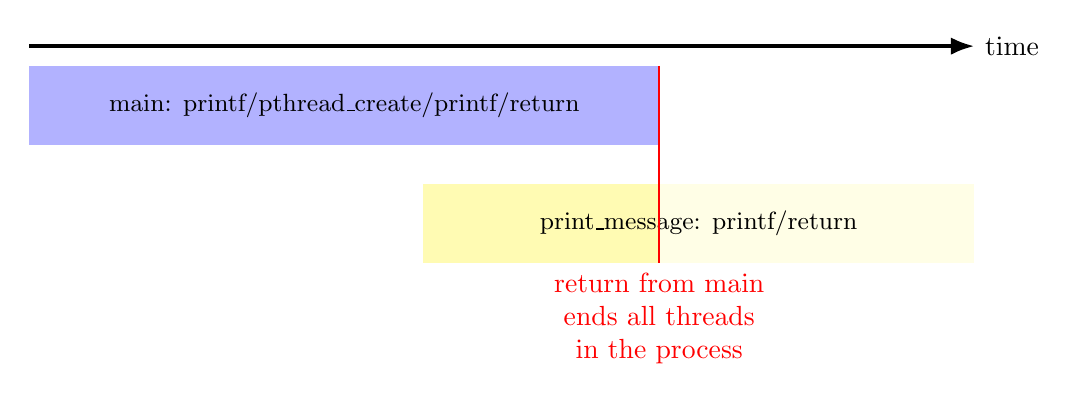
\begin{tikzpicture}
\tikzset{
    box/.style={draw,thick},
    main box/.style={fill=blue!30},
    thread box/.style={fill=yellow!30},
    my label/.style={font=\small},
    >=Latex,
}
\draw[very thick,->] (0,1.25) -- (12,1.25) node[right] {time};
\path[main box] (0, 0) rectangle (8, 1) node[midway,my label]{main: printf/pthread\_create/printf/return};
\path[thread box] (5, -.5) rectangle (8, -1.5);
\path[thread box,fill=yellow!10,dashed] (8, -.5) rectangle (12, -1.5);
\path (5, -.5) rectangle (12, -1.5) node[midway,my label]{print\_message: printf/return};
\path[draw,thick,red] (8, 1) -- (8,-1.5) node[below,align=center] {return from main \\ ends all threads \\ in the process};
\end{tikzpicture}
\end{frame}


\againframe<1>{pthreadCreateBrokenP}

\againframe<1>{pthreadCreateRace}
\begin{frame}{the correctness problem}
\begin{itemize}
\item schedulers introduce non-determinism
    \begin{itemize}
    \item scheduler might run threads in \myemph{any order}
    \item scheduler can switch threads at \myemph{any time}
    \end{itemize}
\item worse with threads on multiple cores
    \begin{itemize}
    \item cores \myemph{not precisely synchronized} (stalling for caches, etc., etc.)
    \item different cores happen in different order each time
    \end{itemize}
\vspace{.5cm}
\item allows for ``race condition'' bugs
    \begin{itemize}
    \item outcome depends on whether one thread can `race' ahead of another
    \end{itemize}
\item \ldots to be avoided by synchronization constructs
    \begin{itemize}
    \item what we'll talk about for a while\ldots
    \end{itemize}
\end{itemize}
\end{frame}


\section{the lost write}

\subsection{motivation: threaded ATM server?}
\usetikzlibrary{fit}
% 

\begin{frame}{example application: ATM server}
\begin{itemize}
    \item commands: withdraw, deposit
    \item one correctness goal: don't lose money
\end{itemize}
\end{frame}

\begin{frame}[fragile,label=serverCode]{ATM server}
\vspace{-.5cm}
{\small (pseudocode)}
\begin{lstlisting}[language=C++,style=small]
ServerLoop() {
    while (true) {
        ReceiveRequest(&operation, &accountNumber, &amount);
        if (operation == DEPOSIT) {
            Deposit(accountNumber, amount);
        } else ...
    }
}
Deposit(accountNumber, amount) {
    account = GetAccount(accountNumber);
    account->balance += amount;
    SaveAccountUpdates(account);
}
\end{lstlisting}
\end{frame}


\begin{frame}[fragile,label=threadedServerLoop]{multiple threads}
\begin{lstlisting}[
    language=C++,
    style=smaller,
    moredelim={**[is][\btHL<1-|handout:1->]{@1}{1@}}
]
main() {
    for (int i = 0; i < NumberOfThreads; ++i) {
        pthread_create(&server_loop_threads[i], NULL,
                       ServerLoop, NULL);
    }
    ...
}

ServerLoop() {
    while (true) {
        ReceiveRequest(&operation, &accountNumber, &amount);
        if (operation == DEPOSIT) {
            Deposit(accountNumber, amount);
        } else ...
    }
}
\end{lstlisting}
\end{frame}


\subsection{example}
\begin{frame}[fragile,label=theLostWrite]{the lost write}
\begin{tikzpicture}
\node[font=\tt\small] (cpp code) {
account->balance += amount;
};
\node[anchor=west] at (cpp code.east) { (in two threads, same account) };
\draw[very thick,dotted] (cpp code.south west) -- ++(15cm,0cm);

\node[font=\tt\small,label={north:Thread A},align=left,anchor=north west] (thread A part 1) at ([yshift=-1cm]cpp code.south west) {
mov account->balance, \%rax \\
add amount, \%rax \\
};
\node[label={north:Thread B},anchor=north west] (thread B top) at ([xshift=.5cm]thread A part 1.north east) {
\hspace{5cm}
};
\node[font=\tt\small,align=left,anchor=north west] (thread B part 1) at (thread B top.west |- thread A part 1.south) {
mov account->balance, \%rax \\
add amount, \%rax \\
};
\node[align=left,font=\tt\small,anchor=north west] (thread A part 2) at (thread A part 1.west |- thread B part 1.south) {
mov \%rax, account->balance \\
};
\node[align=left,anchor=north west,font=\tt\small] (thread B part 2) at (thread B part 1.west |- thread A part 2.south) {
mov \%rax, account->balance
};
\foreach \place in {thread A part 1,thread B part 1,thread A part 2} {
    \draw[ultra thick] (\place.south -| thread A part 1.west) -- (\place.south -| thread B part 1.east)
        node[midway,fill=white,font=\small]{context switch};
}
\begin{visibleenv}<2->
    \node[draw,red,ultra thick,fit=(thread A part 2),
        label={[red]south:lost write to balance}] {};
    \node[draw,blue,ultra thick,fit=(thread B part 2),
        label={[blue]south:``winner'' of the race}] {};
\end{visibleenv}
\begin{visibleenv}<3->
    \node[draw,red,ultra thick,anchor=north,fill=white] at ([xshift=-3cm,yshift=-0.5cm]thread B part 2.south west) {
        lost track of thread A's money
    };
\end{visibleenv}
\end{tikzpicture}
\end{frame}


\section{race conditions and atomicity}
\subsection{thinking about simple races} 
\begin{frame}{thinking about race conditions (1)}
\begin{itemize}
\item what are the possible values of $x$? (initially $x = y = 0$)  \\
\begin{tabular}{cc}
    \bfseries{Thread A} & \bfseries{Thread B} \\ \hline
    $x \leftarrow 1$ & $y \leftarrow 2$ \\
\end{tabular}
\iftoggle{heldback}{}{
\item<2-> must be 1. Thread B can't do anything
}
\end{itemize}
\end{frame}

\begin{frame}<1-2>[label=thinkRace2]{thinking about race conditions (2)}
\begin{itemize}
\item possible values of $x$? (initially $x = y = 0$) \\
\begin{tabular}{cc}
    \bfseries{Thread A} & \bfseries{Thread B} \\ \hline
    $x \leftarrow y + 1$ & $y \leftarrow 2$ \\
                    ~ & $y \leftarrow y \times 2$ \\
\end{tabular}
\iftoggle{heldback}{}{
\item<2-> if A goes first, then B: $1$
\item<2-> if B goes first, then A: $5$
\item<2-> if B line one, then A, then B line two: $3$
\item<3-> \ldots and why not 7:
    \begin{itemize}
    \item B (start): $y \leftarrow 2 = 0010_{\text{TWO}}$; then y bit 3 $\leftarrow$ 0; y bit 2 $\leftarrow$ 1; then
    \item A: x $\leftarrow 110_{\text{TWO}} + 1 = 7$; then
    \item B (finish): y bit 1 $\leftarrow$ 0; y bit 0 $\leftarrow$ 0
    \end{itemize}
}
\end{itemize}
\end{frame}

\begin{frame}{thinking about race conditions (3)}
\begin{itemize}
\item what are the possible values of $x$? \\
\item (initially $x = y = 0$) \\
\begin{tabular}{cc}
    \bfseries{Thread A} & \bfseries{Thread B} \\ \hline
    $x \leftarrow 1$ & $x \leftarrow 2$ \\
\end{tabular}
\iftoggle{heldback}{}{
\item<2-> 1 or 2
\item<3-> \ldots but why not 3?
    \begin{itemize}
    \item B: x bit 0 $\leftarrow 0$
    \item A: x bit 0 $\leftarrow 1$
    \item A: x bit 1 $\leftarrow 0$
    \item B: x bit 1 $\leftarrow 1$
    \end{itemize}
}
\end{itemize}
\end{frame}

\againframe<3>{thinkRace2}


\subsection{atomicity definition}
\begin{frame}{atomic operation}
\begin{itemize}
\item \textit{atomic operation} = operation that runs to completion or not at all
\item we will use these to let threads work together
\vspace{.5cm}
\item most machines: loading/storing {\small (aligned)} words is atomic
    \begin{itemize}
    \item so can't get $3$ from $x \leftarrow 1$ and $x \leftarrow 2$ running in parallel
    \item aligned $\approx$ address of word is multiple of word size (typically done by compilers)
    \end{itemize}
\item but some instructions are not atomic; examples:
    \begin{itemize}
    \item x86: integer \texttt{add} constant to memory location
    \item many CPUs: loading/storing values that cross cache blocks
        \begin{itemize}
            \item e.g. if cache blocks \texttt{0x40} bytes, load/store 4 byte from addr. \texttt{0x3E} is not atomic
        \end{itemize}
    \end{itemize}
\end{itemize}
\end{frame}



\subsection{example: x86 add not atomic}

\begin{frame}[fragile,label=lostAdds]{lost adds (program)}
\begin{lstlisting}[language=myasm,style=smaller]
.global update_loop
update_loop:
    addl $1, the_value // the_value (global variable) += 1
    dec %rdi           // argument 1 -= 1
    jg update_loop     // if argument 1 >= 0 repeat
    ret
\end{lstlisting}
\hrule
\begin{lstlisting}[language=C++,style=smaller]
int the_value;
extern void *update_loop(void *);
int main(void) {
    the_value = 0;
    pthread_t A, B;
    pthread_create(&A, NULL, update_loop, (void*) 1000000);
    pthread_create(&B, NULL, update_loop, (void*) 1000000);
    pthread_join(A, NULL);
    pthread_join(B, NULL);
    // expected result: 1000000 + 1000000 = 2000000
    printf("the_value = %d\n", the_value);
}
\end{lstlisting}
\end{frame}

\begin{frame}[fragile,label=lostAddsResult]{lost adds (results)}
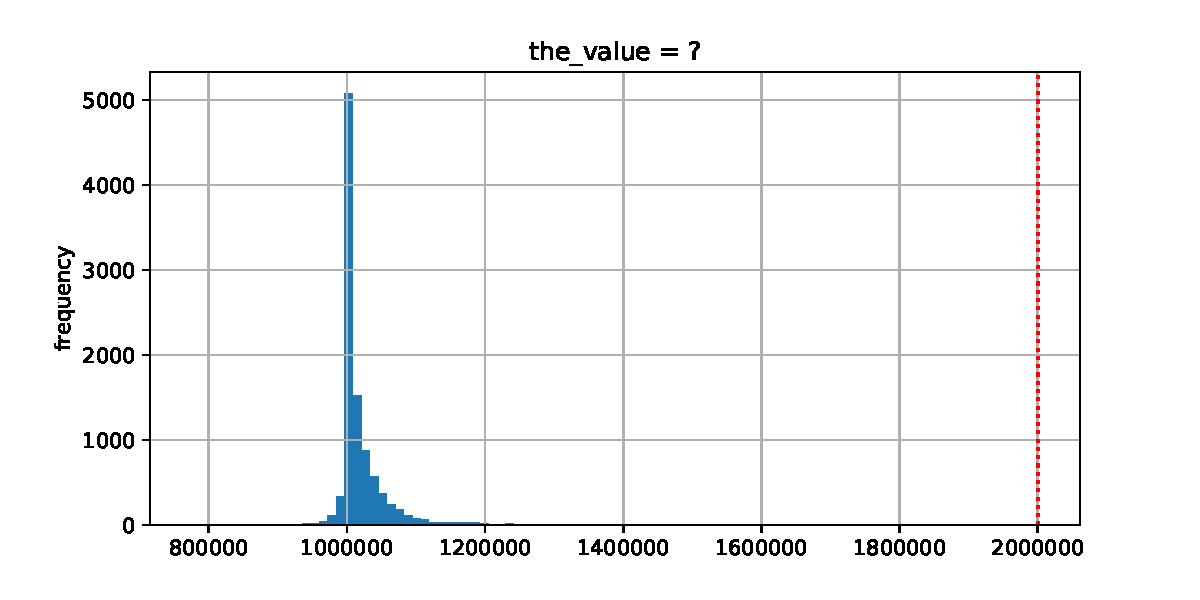
\includegraphics[width=1.1\textwidth]{../sync/parallel-add-histogram}
\end{frame}

\begin{frame}{but how?}
    \begin{itemize}
    \item probably not possible on single core
        \begin{itemize}
            \item exceptions can't occur in the middle of \texttt{add} instruction
        \end{itemize}
    \item \ldots but `add to memory' implemented with multiple steps
        \begin{itemize}
        \item still needs to load, add, store internally
        \item can be interleaved with what other cores do
        \end{itemize}
        \vspace{.5cm}
    \item<2-> {\small (and actually it's more complicated than that --- we'll talk later)}
    \end{itemize}
\end{frame}



\subsection{what is atomic?}

\begin{frame}{so, what is actually atomic}
    \begin{itemize}
    \item for now we'll assume: load/stores of `words' 
        \begin{itemize}
        \item  (64-bit machine = 64-bits words)
        \end{itemize}
        \vspace{.5cm}
    \item in general: \myemph{processor designer will tell you}
    \item their job to design caches, etc. to work as documented
    \end{itemize}
\end{frame}


\section{read-modify-write atomic operations}
\begin{frame}{atomic read-modfiy-write}
    \begin{itemize}
    \item really hard to build locks for atomic load store
        \begin{itemize}
        \item and normal load/stores aren't even atomic\ldots
        \end{itemize}
    \item \ldots so processors provide \myemph{read/modify/write} operations
        \vspace{.5cm}
    \item one instruction that\\\textit{atomically}\\reads \textit{and} modifies \textit{and} writes back a value
    \vspace{.5cm}
    \item used by OS to implement higher-level synchronization tools
    \end{itemize}
\end{frame}

\subsection{x86 atomic exchange} 
\begin{frame}[fragile,label=atomicXchg]{x86 atomic exchange}
\begin{lstlisting}[language=myasm]
lock xchg (%ecx), %eax
\end{lstlisting}
\begin{itemize}
    \item atomic exchange
    \item \texttt{temp $\leftarrow$ M[ECX]}
    \item \texttt{M[ECX] $\leftarrow$ EAX}
    \item \texttt{EAX $\leftarrow$ temp}
    \item \ldots without being interrupted by other processors, etc.
\end{itemize}
\end{frame}


\begin{frame}{implementing atomic exchange}
    \begin{itemize}
    \item make sure other processors don't have cache block
    \begin{itemize}
        \item probably need to be able to do this to keep caches in sync
    \end{itemize}
    \item do read+modify+write operation
    \end{itemize}
\end{frame}



\section{definitions: mutual exclusion, critical section}
\begin{frame}{some definitions}
\begin{itemize}
\item \textbf{mutual exclusion}: ensuring only one thread does a particular thing at a time
    \begin{itemize}
        \item like updating shared balance
    \end{itemize}
\item<2-> \textbf{critical section}: code that exactly one thread can execute at a time
    \begin{itemize}
        \item result of mutual exclusion
    \end{itemize}
\item<3-> \textbf{lock}: object only one thread can hold at a time
    \begin{itemize}
        \item interface for creating critical sections
    \end{itemize}
\end{itemize}
\end{frame}


\section{locks}
\begin{frame}{lock analogy}
    \begin{itemize}
    \item agreement: whoever holds the flag can access shared resource
        \begin{itemize}
        \item flag doesn't actually do anything by itself\ldots
        \end{itemize}
    \item acquire/lock $\approx$ wait for and grab flag from table
    \item release/unlock $\approx$ put flag back on table
    \vspace{.5cm}
    \item<2-> agreement is \myemph{voluntary}
        \begin{itemize}
        \item thread tries to manipulate shared resource without lock? \\
            lock won't stop it\ldots
        \end{itemize}
    \item<2-> lock is \textit{held} by particular thread
    \end{itemize}
\end{frame}


% FIXME: lock analogy: hat
\begin{frame}[fragile,label=lockDefn]{the lock primitive}
    \begin{itemize}
    \item locks: an object with (at least) two operations:
        \begin{itemize}
        \item \textit{acquire} or \textit{lock} --- wait until lock is free, then ``grab'' it
        \item \textit{release} or \textit{unlock} --- let others use lock, wakeup waiters
        \end{itemize}
    \item typical usage: everyone acquires lock before using shared resource
        \begin{itemize}
        \item forget to acquire lock? weird things happen
        \end{itemize}
    \end{itemize}
\begin{lstlisting}[language=C++,style=small]
Lock(account_lock);
balance += ...;
Unlock(account_lock);
\end{lstlisting}
\end{frame}


\begin{frame}[fragile,label=pthreadMutex]{pthread mutex}
\begin{lstlisting}[language=C++,style=small]
#include <pthread.h>

pthread_mutex_t account_lock;
pthread_mutex_init(&account_lock, NULL);
    // or: pthread_mutex_t account_lock =
    //              PTHREAD_MUTEX_INITIALIZER;
...
pthread_mutex_lock(&account_lock);
balance += ...;
pthread_mutex_unlock(&account_lock;
\end{lstlisting}
\end{frame}



\subsection{exercise}
\begin{frame}[fragile,label=lockEx]{exercise}
    \vspace{-0.5cm}
\begin{lstlisting}[style=smaller]
pthread_mutex_t lock1 = PTHREAD_MUTEX_INITIALIZER;
pthread_mutex_t lock2 = PTHREAD_MUTEX_INITIALIZER;
string one = "init one", two = "init two";
void ThreadA() {
    pthread_mutex_lock(&lock1);
    one = "one in ThreadA";  // (A1)
    pthread_mutex_unlock(&lock1);
    pthread_mutex_lock(&lock2);
    two = "two in ThreadA";  // (A2)
    pthread_mutex_unlock(&lock2);
}
void ThreadB() {
    pthread_mutex_lock(&lock1);
    one = "one in ThreadB";  // (B1)
    pthread_mutex_lock(&lock2);
    two = "two in ThreadB";  // (B2)
    pthread_mutex_unlock(&lock2);
    pthread_mutex_unlock(&lock1);
}
\end{lstlisting}
possible values of one/two after A+B run?
\end{frame}

\begin{frame}<0>[fragile,label=lockExSln]{solution}
\begin{itemize}
\item B1+A2
    \begin{itemize}
    \item A: L(1) A1 U(1) L
    \item B: L(1) B1 L(2) B2 U(2) U(1)
    \item A: L(2) A2 U(2)
    \end{itemize}
\item NOT A1+B2
    \begin{itemize}
    \item would need to run B1 after A1 before A2
    \item not possible because Lock1 held for entire B1+B2 operation
    \item \ldots and A1 needs Lock1, too
    \end{iteimze}
\end{itemize}
\end{frame}

\begin{frame}[fragile,label=lockExAlt1]{exercise (alternate 1)}
    \vspace{-0.5cm}
\begin{lstlisting}[style=smaller]
pthread_mutex_t lock1 = PTHREAD_MUTEX_INITIALIZER;
pthread_mutex_t lock2 = PTHREAD_MUTEX_INITIALIZER;
string one = "init one", two = "init two";
void ThreadA() {
    pthread_mutex_lock(&lock2);
    two = "two in ThreadA";  // (A2)
    pthread_mutex_unlock(&lock2);
    pthread_mutex_lock(&lock1);
    one = "one in ThreadA";  // (A1)
    pthread_mutex_unlock(&lock1);
}
void ThreadB() {
    pthread_mutex_lock(&lock1);
    one = "one in ThreadB";  // (B1)
    pthread_mutex_lock(&lock2);
    two = "two in ThreadB";  // (B2)
    pthread_mutex_unlock(&lock2);
    pthread_mutex_unlock(&lock1);
}
\end{lstlisting}
possible values of one/two after A+B run?
\end{frame}

\begin{frame}[fragile,label=lockExAlt2]{exercise (alternate 2)}
    \vspace{-0.5cm}
\begin{lstlisting}[style=smaller]
pthread_mutex_t lock1 = PTHREAD_MUTEX_INITIALIZER;
pthread_mutex_t lock2 = PTHREAD_MUTEX_INITIALIZER;
string one = "init one", two = "init two";
void ThreadA() {
    pthread_mutex_lock(&lock2);
    two = "two in ThreadA";  // (A2)
    pthread_mutex_unlock(&lock2);
    pthread_mutex_lock(&lock1);
    one = "one in ThreadA";  // (A1)
    pthread_mutex_unlock(&lock1);
}
void ThreadB() {
    pthread_mutex_lock(&lock1);
    one = "one in ThreadB";  // (B1)
    pthread_mutex_unlock(&lock1);
    pthread_mutex_lock(&lock2);
    two = "two in ThreadB";  // (B2)
    pthread_mutex_unlock(&lock2);
}
\end{lstlisting}
possible values of one/two after A+B run?
\end{frame}


\subsection{pthread\_mutex: lock where you unlock}
\begin{frame}{POSIX mutex restrictions}
\begin{itemize}
\item pthread\_mutex rule: \myemph{unlock from same thread you lock in}
\vspace{.5cm}
\item does this actually matter?
\item depends on how pthread\_mutex is implemented
\end{itemize}
\end{frame}


\section{preview: beyond locks}
\begin{frame}{are locks enough?}
\begin{itemize}
    \item do we need more than locks?
\end{itemize}
\end{frame}

\begin{frame}{example 1: pipes?}
\begin{itemize}
\item suppose we want to implement a pipe with threads
\item \texttt{read} sometimes needs to wait for a \texttt{write}
\item don't want busy-wait
\begin{itemize}
\item (and trick of having writer unlock() so reader can finish a lock() is illegal)
\end{itemize}
\end{itemize}
\end{frame}

\begin{frame}{more synchronization primitives}
    \begin{itemize}
    \item need other ways to wait for threads to finish
    \item we'll introduce several synchronization ideas beyond locks:
        \begin{itemize}
        \item barriers --- (today)
        \item condition variables / monitors
        \item counting semaphores
        \item reader/writer locks
        \end{itemize}
    \end{itemize}
\end{frame}



\section{barriers}
\begin{frame}{barriers}
\begin{itemize}
\item compute minimum of 100M element array with 2 processors
\item algorithm:
\vspace{.5cm}
\item compute minimum of 50M of the elements on each CPU
    \begin{itemize}
    \item one thread for each CPU
    \end{itemize}
\item \myemph<2>{wait for all computations to finish}
\item take minimum of all the minimums
\end{itemize}
\end{frame}

\begin{frame}[fragile,label=barrierAPI]{barriers API}
\begin{itemize}
\item barrier.Initialize(NumberOfThreads)
\item barrier.Wait() --- return after all threads have waited
\vspace{.5cm}
\item idea: multiple threads perform computations in parallel
\item threads wait for \myemph{all other threads} to call Wait()
\end{itemize}
\end{frame}

\begin{frame}[fragile,label=barrierWait]{barrier: waiting for finish}
\begin{tikzpicture}
\node[label={north:Thread 0}] (code one) {
\begin{lstlisting}[language=C++,style=smaller]
partial_mins[0] = 
    /* min of first
       50M elems */;

barrier.Wait();


total_min = min(
    partial_mins[0],
    partial_mins[1]
);
\end{lstlisting}
};
\node[anchor=south] (code zero) at ([yshift=1cm]code one.north) {
\begin{lstlisting}[language=C++,style=smaller]
barrier.Initialize(2);
\end{lstlisting}
};

\node[label={north:Thread 1},anchor=north west] (code two) at ([xshift=1cm]code one.north east) {
\begin{lstlisting}[language=C++,style=smaller]


partial_mins[1] =
    /* min of last
       50M elems */
barrier.Wait();
\end{lstlisting}
};
\end{tikzpicture}
\end{frame}

\begin{frame}[fragile,label=barrierReuse]{barriers: reuse}
\begin{tikzpicture}
\node[label={north:Thread 0}] (code one) {
\begin{lstlisting}[
    language=C++,style=smaller,
    moredelim={**[is][\btHL<2|handout:0>]{@2}{2@}},
    moredelim={**[is][\btHL<3|handout:0>]{@3}{3@}},
    moredelim={**[is][\btHL<3|handout:0>]{@4}{4@}},
]
@2results[0][0]2@ = getInitial(0);
barrier.Wait();

@4results[1][0]4@ =
    computeFrom(0, 
        results[0][0],
        @3results[0][1]3@
    );
barrier.Wait();

results[2][0] =
    computeFrom(0,
        results[1][0],
        results[1][1]
    );
\end{lstlisting}
};
\node[label={north:Thread 1},anchor=north west] (code two) at ([xshift=1cm]code one.north east) {
\begin{lstlisting}[
    language=C++,style=smaller,
    moredelim={**[is][\btHL<2|handout:0>]{@2}{2@}},
    moredelim={**[is][\btHL<3|handout:0>]{@3}{3@}},
    moredelim={**[is][\btHL<3|handout:0>]{@4}{4@}},
]
@3results[0][1]3@ = getInitial(1);
barrier.Wait();

results[1][1] =
    computeFrom(1, 
        @2results[0][0],2@
        results[0][1]
    );
barrier.Wait();

results[2][1] =
    computeFrom(1,
        @4results[1][0]4@,
        results[1][1]
    );
\end{lstlisting}
};
\end{tikzpicture}
\end{frame}

\begin{frame}[fragile,label=pthreadBarrier]{pthread barriers}
\begin{lstlisting}[language=C++,style=smaller]
pthread_barrier_t barrier;
pthread_barrier_init(
    &barrier,
    NULL /* attributes */,
    numberOfThreads
);
...
...
pthread_barrier_wait(&barrier);
\end{lstlisting}
\end{frame}



\section{life HW}
\begin{frame}[fragile,label=lifeHW]{life homework (pseudocode)}
\begin{lstlisting}[
    language=C++,style=smaller,
    moredelim={**[is][\btHL<2|handout:0>]{@2}{2@}},
    moredelim={**[is][\btHL<3|handout:0>]{@3}{3@}},
    moredelim={**[is][\btHL<3|handout:0>]{@4}{4@}},
]
for (int time = 0; time < MAX_ITERATIONS; ++time) {
    for (int y = 0; y < size; ++y) {
        for (int x = 0; x < size; ++x) {
            to_grid(x, y) = computeValue(from_grid, x, y);
        }
    }
    swap(from_grid, to_grid);
}
\end{lstlisting}
\end{frame}

\begin{frame}{life homework}
\begin{itemize}
\item compute grid of values for time $t$ from grid for time $t-1$
    \begin{itemize}
    \item compute new value at $i,j$ based on surrounding values
    \end{itemize}
\vspace{.5cm}
\item parallel version: produce parts of grid in different threads
\item use barriers to finish time $t$ before going to time $t+1$
\end{itemize}
\end{frame}




\section{preview: more advance sync}
\begin{frame}{preview: general sync}
    \begin{itemize}
    \item lots of coordinating threads beyond locks/barriers
    \item will talk about two general tools later:
        \begin{itemize}
        \item monitors/condition variables
        \item semaphores
        \end{itemize}
    \item big added feature: wait for arbitrary thing to happen
    \end{itemize}
\end{frame}

\begin{frame}[fragile]{a bad idea}
\begin{itemize}
\item one \myemph{bad} idea to wait for an event:
\end{itemize}
\begin{lstlisting}
bool happened = false;
void WaitForEvent() {
    do {} while (!happened);
}

void EventHappened() {
    happened = true;
}
\end{lstlisting}
\begin{itemize}
\item wastes processor time
\item and also \myemph{doesn't work!}
\end{itemize}
\end{frame}


\section{revisiting atomicity}
\subsection{compiler reordering}
\begin{frame}[fragile,label=compReorder]{compilers move loads/stores (1)}
\begin{lstlisting}[language=C++,style=small,
    moredelim={**[is][\btHL<2|handout:2>]{@2}{2@}},
    moredelim={**[is][\btHL<3|handout:3>]{@3}{3@}},
    moredelim={**[is][\btHL<4|handout:4>]{@4}{4@}},
    moredelim={**[is][\btHL<5|handout:5>]{@5}{5@}},
]
void Alice() {
    note_from_alice = 1;
    @2do {} while (note_from_bob);2@
    if (no_milk) {++milk;}
}
\end{lstlisting}
\hrule
\begin{lstlisting}[language=myasm,style=small,
    moredelim={**[is][\btHL<2|handout:2>]{@2}{2@}},
    moredelim={**[is][\btHL<3|handout:3>]{@3}{3@}},
    moredelim={**[is][\btHL<4|handout:4>]{@4}{4@}},
    moredelim={**[is][\btHL<5|handout:5>]{@5}{5@}},
]
Alice:
  movl $1, note_from_alice  // note_from_alice <- 1
  movl note_from_bob, %eax  // eax <- note_from_bob
.L2:
  @2testl %eax, %eax2@
  @2jne .L22@                   // while (eax == 0) repeat
  cmpl $0, no_milk          // if (no_milk != 0) ...
  ...
\end{lstlisting}
\end{frame}

\begin{frame}[fragile,label=compReorder2]{compilers move loads/stores too (2)}
\begin{lstlisting}[language=C++,style=small,
    moredelim={**[is][\btHL<2|handout:2>]{@2}{2@}},
    moredelim={**[is][\btHL<3|handout:3>]{@3}{3@}},
    moredelim={**[is][\btHL<4|handout:4>]{@4}{4@}},
    moredelim={**[is][\btHL<5|handout:5>]{@5}{5@}},
]
void Alice() {
    @3note_from_alice = 1;3@  // "Alice waiting" signal for Bob()
    do {} while (note_from_bob);
    if (no_milk) {++milk;}
    @2note_from_alice = 2;2@
}
\end{lstlisting}
\hrule
\begin{lstlisting}[language=myasm,style=small,
    moredelim={**[is][\btHL<2|handout:2>]{@2}{2@}},
    moredelim={**[is][\btHL<3|handout:3>]{@3}{3@}},
    moredelim={**[is][\btHL<4|handout:4>]{@4}{4@}},
    moredelim={**[is][\btHL<5|handout:5>]{@5}{5@}},
]
Alice:  
  // compiler optimization: don't set note_from_alice to 1,
  // (why? it will be set to 2 anyway)
  @3movl note_from_bob, %eax3@  // eax <- note_from_bob
.L2:
  testl %eax, %eax          
  jne .L2                   // while (eax == 0) repeat
  ...
  @2movl $2, note_from_alice2@  // note_from_alice <- 2
\end{lstlisting}
\end{frame}


\subsection{fix compiler reordering}
\begin{frame}{fixing compiler reordering?}
    \begin{itemize}
    \item isn't there a way to tell compiler not to do these optimizations?
    \item yes, but that is not enough!
    \end{itemize}
\end{frame}

\subsection{processor reordering}
\begin{frame}[fragile,label=loadReorderSetup]{a simple race}
\begin{tikzpicture}
\node (thread A code) {
\begin{lstlisting}[language=myasm,style=smaller]
thread_A:
    movl $1, x   /* x <- 1 */
    movl y, %eax /* return y */
    ret
\end{lstlisting}
};
\node[anchor=north west] (thread B code) at ([xshift=.5cm]thread A code.north east) {
\begin{lstlisting}[language=myasm,style=smaller]
thread_B:
    movl $1, y   /* y <- 1 */
    movl x, %eax /* return x */
    ret
\end{lstlisting}
};
\node[anchor=north](driver code) at ([yshift=-.25cm,xshift=-.25cm]thread B code.south west) {
\begin{lstlisting}[language=C++,style=smaller]
x = y = 0;
pthread_create(&A, NULL, thread_A, NULL);
pthread_create(&B, NULL, thread_B, NULL);
pthread_join(A, &A_result); pthread_join(B, &B_result);
printf("A:%d B:%d\n", (int) A_result, (int) B_result);
\end{lstlisting}
};
\end{tikzpicture} 
\begin{itemize}
\item<2-> if loads/stores atomic, then possible results:
    \begin{itemize}
    \item A:1 B:1 --- both moves into x and y, then both moves into eax execute
    \item A:0 B:1 --- thread A executes before thread B
    \item A:1 B:0 --- thread B executes before thread A
    \end{itemize}
\end{itemize}
\end{frame}

\begin{frame}[fragile,label=loadReorderExpResults]{a simple race: results}
\begin{tikzpicture}
\node (thread A code) {
\begin{lstlisting}[language=myasm,style=smaller]
thread_A:
    movl $1, x   /* x <- 1 */
    movl y, %eax /* return y */
    ret
\end{lstlisting}
};
\node[anchor=north west] (thread B code) at ([xshift=.5cm]thread A code.north east) {
\begin{lstlisting}[language=myasm,style=smaller]
thread_B:
    movl $1, y   /* y <- 1 */
    movl x, %eax /* return x */
    ret
\end{lstlisting}
};
\node[anchor=north] (driver code) at ([yshift=-.25cm,xshift=-.25cm]thread B code.south west) {
\begin{lstlisting}[language=C++,style=smaller]
x = y = 0;
pthread_create(&A, NULL, thread_A, NULL);
pthread_create(&B, NULL, thread_B, NULL);
pthread_join(A, &A_result); pthread_join(B, &B_result);
printf("A:%d B:%d\n", (int) A_result, (int) B_result);
\end{lstlisting}
};
\end{tikzpicture} 
\begin{center}
\small my desktop, 100M trials: \\
\begin{tabular}{r|l|l}
frequency & result & ~ \\ \hline
$99\,823\,739$ & A:0 B:1 & (`A executes before B') \\
$171\,161$& A:1 B:0 & (`B executes before A') \\
$4\,706$ & A:1 B:1 & (`execute moves into x+y first') \\
\myemph<2>{$394$} & \myemph<2>{A:0 B:0} & \myemph<2>{???} \\
\end{tabular}
\end{center}
\end{frame}


\subsection{why reorder?}

\begin{frame}[fragile]{why reorder here?}
\begin{tikzpicture}
\node (thread A code) {
\begin{lstlisting}[language=myasm,style=smaller]
thread_A:
    movl $1, x   /* x <- 1 */
    movl y, %eax /* return y */
    ret
\end{lstlisting}
};
\node[anchor=north west] (thread B code) at ([xshift=.5cm]thread A code.north east) {
\begin{lstlisting}[language=myasm,style=smaller]
thread_B:
    movl $1, y   /* y <- 1 */
    movl x, %eax /* return x */
    ret
\end{lstlisting}
};
\end{tikzpicture}
\begin{itemize}
\item thread A: faster to load \texttt{y} right now!
\item \ldots rather than wait for write of \texttt{x} to finish
\end{itemize}
\end{frame}


\usetikzlibrary{calc}

\begin{frame}{load/store reordering}
\begin{itemize}
    \item load/stores atomic, but run \textit{out of order}
    \vspace{.5cm}
    \item recall?: out-of-order processors
    \item processor optimization: sometimes execute instructions in non-program order
        \begin{itemize}
        \item hide delays from slow caches, variable computation rates, etc.
        \item documneted limits on when this is/is not allowed
        \end{itemize}
    \item track side-effects \textit{within a thread} to make as if in-order
        \begin{itemize}
        \item but common choice: don't worry as much between cores/threads
        \item design decision: if programmer cares, they worry about it
        \end{itemize}
    \item want to avoid this \textit{special instructions ensure strict ordering}
\end{itemize}
\end{frame}

\begin{frame}{why load/store reordering?}
\begin{itemize}
\item prior example: load of x executing before store of y
\item why do this? otherwise delay the load
    \begin{itemize}
    \item if x and y unrelated --- no benefit to waiting
    \end{itemize}
\end{itemize}
\end{frame}





\section{pthreads and load/store reordering}
\begin{frame}{pthreads and reordering}
    \begin{itemize}
    \item many pthreads functions \myemph{prevent reordering}
        \begin{itemize}
        \item everything before function call actually happens before 
        \end{itemize}
    \item includes \myemph{preventing some optimizations}
        \begin{itemize}
        \item e.g. keeping global variable in register for too long
        \end{itemize}
    \vspace{.5cm}
    \item pthread\_create, pthread\_join, other tools we'll talk about \ldots
        \begin{itemize}
        \item basically: if pthreads is waiting for/starting something, no weird ordering
        \end{itemize}
    \item implementation part 1: prevent compiler reordering
    \item implementation part 2: use special instructions
        \begin{itemize}
        \item example: x86 \texttt{mfence} instruction
        \end{itemize}
    \end{itemize}
\end{frame}



